%-------------------------------------------------------------------------------
\subsubsection{Barycentre et médiane géométrique}
%-------------------------------------------------------------------------------

On considère $n$ points $x_1, \dots x_n$ de $\Rbb^d$ et on cherche à définir un point central $m$ du ``nuage de points'' $(x_i)_{1 \leq i \leq n}$. On notera $(x_{ij})_{1 \leq j \leq d}$ les coordonnées points $x_i$. 

\paragraph{Barycentre.}
On considère tout d'abord la fonction
$$
\begin{array}{rlcl}
  f: & \Rbb^d & \mapsto & \Rbb^+ \\
  & y & \to & f(y) = \sum_{i=1}^n \|x_i - y\|_2^2
  \end{array}
$$
où $\|u\|_2$ désigne la norme euclidienne: $\|u\|_2 = \sqrt{\sum_{j=1}^n u_j^2}$.

\begin{enumerate}
  \item Montrer que la fonction $f$ admet un unique minimum $y^*$ qui est le barycentre des points $(x_i)_{1 \leq i \leq n}$, c'est à dire, 
  $$
  y^* = (y^*_j)_{1 \leq j \leq d}, 
  \qquad
  y^*_j = \frac1n \sum_{i=1}^n x_{ij}
  $$
  \solution{
    Le jacobien de $f$ au point $y$ est
    $$
    J_y f = \left[2 \sum_i (y_j - x_{ij})\right]_{1 \leq j \leq d}
    $$
    dont les éléments s'annulent respectivement uniquement pour
    $$
    y^*_j = \frac1n \sum_{i=1}^n x_{ij}.
    $$
    On vérifie qu'il s'agit d'un minimum en déterminant la hessienne de $f$ au point $y^*$:
    $$
    \nabla^2_{y^*} f = 2 I_d
    $$
    qui est bien strictement définie positive.
  }
\end{enumerate}

\paragraph{Fonction convexe.}
On rappelle qu'une fonction $h: \Rbb^d \mapsto \Rbb$ est convexe si et seulement si pour tout couple $(u, v)$ et tout réel $0 < a < 1$, on a
$$
h(au + (1-a) v) \leq a h(u) + (1-a) h(v).
$$
La fonction est strictement convexe si l'inégalité est stricte pour pour tout $0 < a < 1$.

\begin{enumerate}
  \setcounter{enumi}{1}  
  \item Montre qu'une fonction $h$ strictement convexe admet un minimum unique.
  \solution{
    On peut raisonner par l'absurde. Si $h$ admet deux minimums $u_1$ et $u_2$ (avec donc $f(u_1) = f(u_2)$), alors pour $0 < a < 1$, on a
    $$
    f(a u_1  +(1 - a) u_2) < a f(u_1) + (1 - a) f(u_2) = f(u_1)
    $$
    ce qui est en contradiction avec le fait que $u_1$ soit un minimum.
  }
\end{enumerate}


\paragraph{Médiane géométrique.}
On considère maintenant la fonction
$$
\begin{array}{rlcl}
  g: & \Rbb^d & \mapsto & \Rbb^+ \\
  & y & \to & f(y) = \sum_{i=1}^n \|x_i - y\|_2
  \end{array}
$$

\begin{enumerate}
  \setcounter{enumi}{2}  
  \item Montrer que $g$ est strictement convexe si les $n$ points $x_1, \dots x_n$ ne sont pas tous alignés.
  \solution{
    Soient $u$ et $v$ deux points de $\Rbb^d$ et $0 < a < 1$, on a 
    \begin{align*}
      f(a u  + (1 - a) v) 
      & = \sum_{i=1}^n \|x_i - a u - (1 - a) v\| \\
      & = \sum_{i=1}^n \|a(x_i - u) + (1 - a)(x_i - v)\| &
      & (\text{car $x_i = a x_i + (1-a) x_i$})\\
      & \leq \sum_{i=1}^n \|a(x_i - u)\| + \|(1 - a)(x_i - v)\| &
      & (\text{par l'inégalité triangulaire}) \\
      & = \sum_{i=1}^n a \|x_i - u\| + (1 - a) \|(x_i - v)\| &
      & (\text{car $a > 0$ et $1 - a > 0$})
    \end{align*}
    donc $g$ est bien convexe. \\
    De plus, on n'a l'égalité
    $$
    \|a(x_i - u) + (1 - a)(x_i - v)\| = \|a(x_i - u)\| + \|(1 - a)(x_i - v)\|
    $$
    que si $u$, $x_i$ et $v$ sont alignés. Si tous les $x_i$ ne sont pas alignés entre eux, pour tout couple $(u, v)$ il existe donc au moins un indice $x_i$ pour lequel l'inégalité triangulaire est stricte, donc
    $$
    \sum_{i=1}^n \|a(x_i - u) + (1 - a)(x_i - v)\| 
    < \sum_{i=1}^n \|a(x_i - u)\| + \|(1 - a)(x_i - v)\|
    $$
    et $g$ est donc strictement convexe.
  }
  \item En déduire que le point $\widetilde{y}$ qui minimise $g$ est unique. On appelle ce point médiane géométrique des points $x_1, \dots x_n$.
  \solution{
    C'est une application directe des deux questions précédentes. \\
    La figure suivante illustre la différence entre le barycentre $y^*$ (en bleu) et la médiane géométrique $\widetilde{y}$ (en rouge) pour $n = 100$ points de $\Rbb^2$. Le point vert $\widehat{y}$ a pour cordonnées respectives les médiane des abscisses et des ordonnées : il ne coincide pas avec la médiane géométrique $\widetilde{y}$.
    $$
    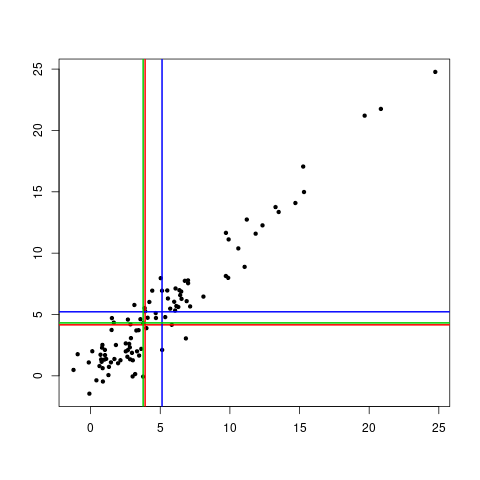
\includegraphics[width=0.4\textwidth, trim=30 30 30 30 30, clip=]{MedianeGeometrique}
    $$
  }
\end{enumerate}
